Entnimmt man einer Spannungsquelle keinen Strom, liegt an den Ausgangsklemmen die Leerlaufspannung $U_0$ an.
Schließt man den Kreislauf, sodass ein endlicher Strom I fließen kann, fällt die Klemmenspannung $U_k$ unter den Wert von $U_0$.
Die Spannungsquelle hat einen Innenwiederstand $R_i$.
Durch das Anschließen eines Messgerätes kommt ein weiterer Widerstand $R_a$, wie in der Abbildung \ref{fig:Monozelle} gezeigt, hinzu. Wegen des Zweiten Kirchhoff'schen Gesetzes gilt
\begin{equation*}
U_0 = IR_i+IR_a
\end{equation*}
\\Da gilt:
\begin{equation}
U_k = IR_a = U_0-IR_i
\label{eqn:klemme}
\end{equation}
\\ist es sinvoll $R_a$ groß zu halten. Somit wird der Strom I klein und es kann
\begin{equation*}
U_k \approx U_0
\end{equation*}
\\angenommen werden.
\\Durch den Innenwiederstand $R_i$ kann man der idealen Spannungsquelle nicht unendlich Leistung entnehmen. Die an $R_a$ abgegebene Leistung lässt sich berechnen mit
\begin{equation*}
  N = I^2R_a.
\end{equation*}
\\Bei der Leistungsanpassung wird ein bestimmtes $R_a$ und I gesucht bei dem N maximal wird.
Bei elektrischen Generatoren ist der Innenwiderstand durch den Rückkopplungsmechanismus festgelegt. Wird der Belastungsstrom geändert, so ändert sich auch das elektrische Verhalten.
Der Innenwiederstand kann hier als differentielle Größe angesehen:
\begin{equation*}
R_i = \frac{dU_k}{dI}.
\end{equation*}
\begin{figure}[h!]
  \centering
  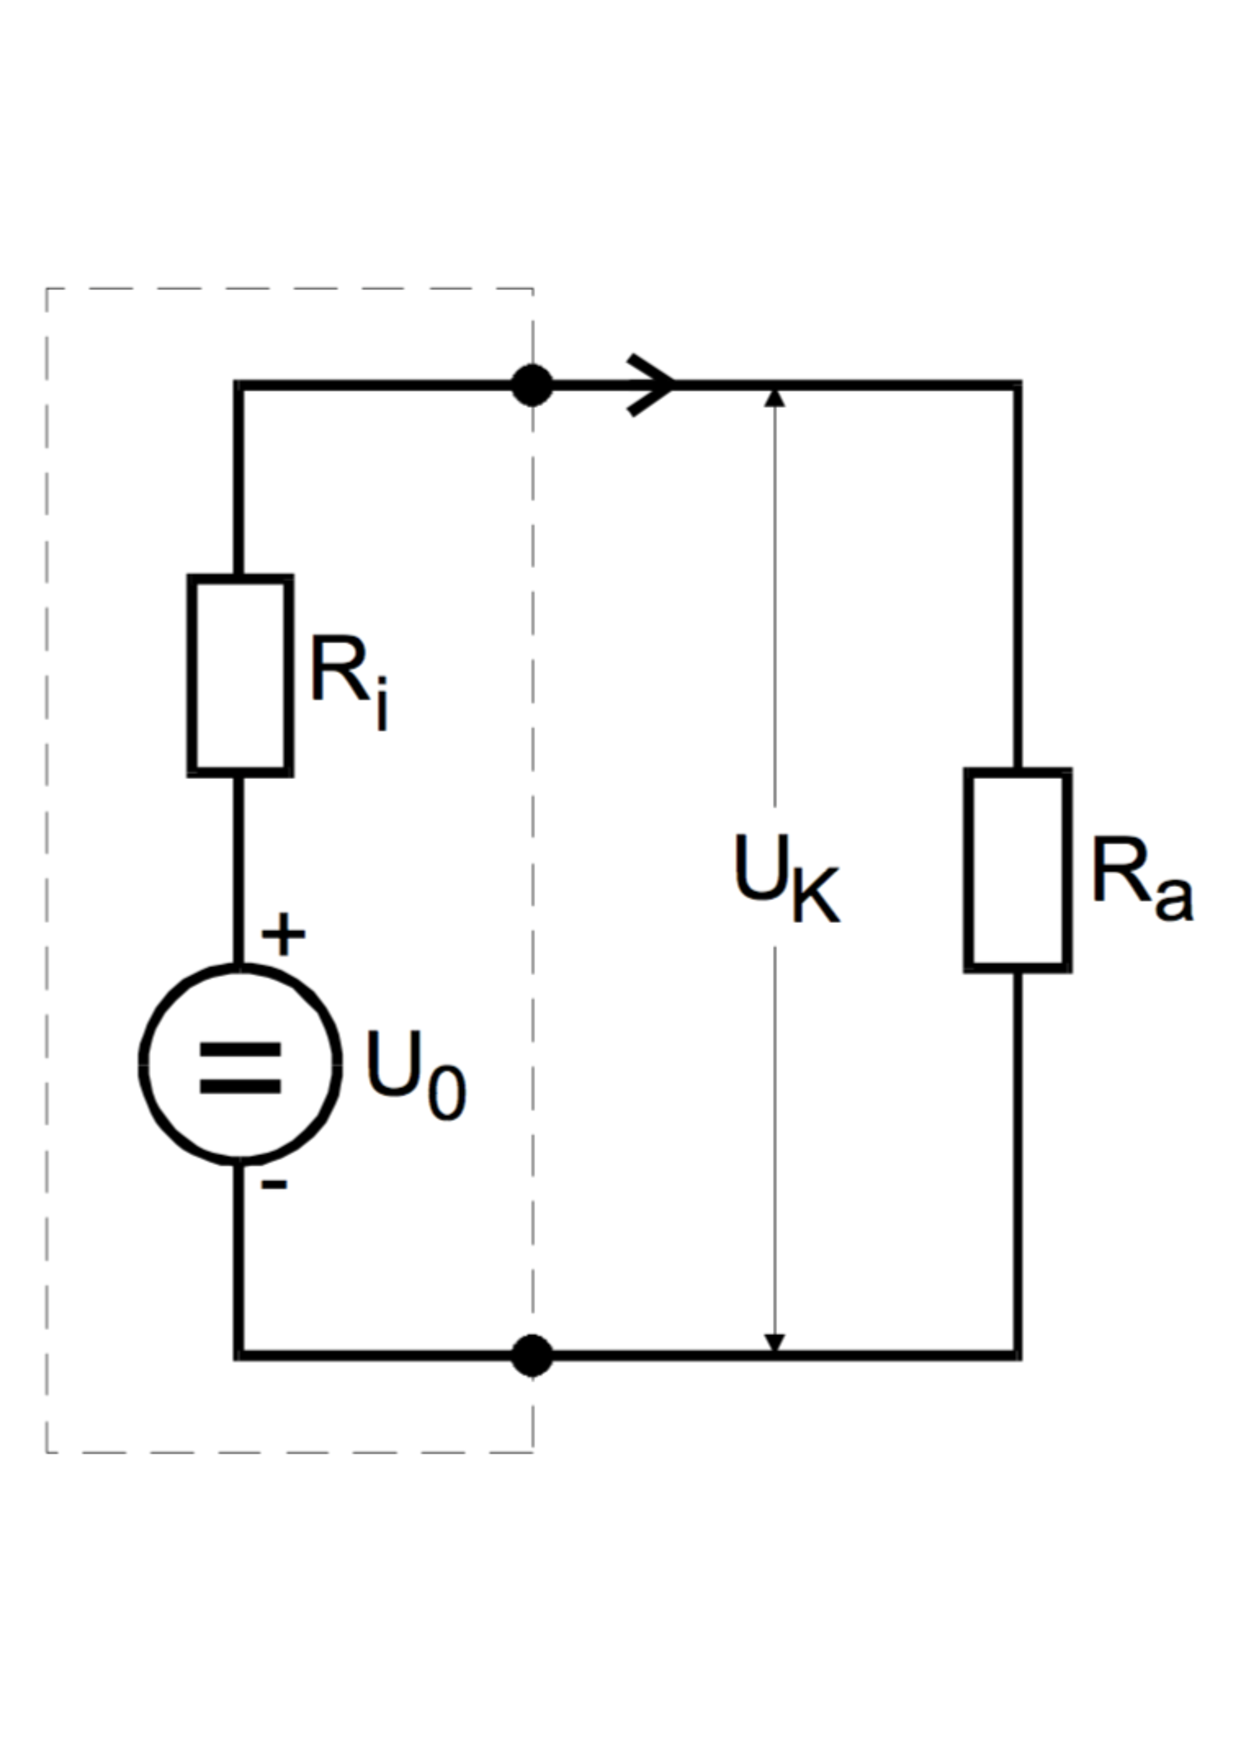
\includegraphics[width=0.7\textwidth]{Monozelle.pdf}
  \caption{Ersatzschaltbild einer realen Spannungsquelle mit Belastungswiderstand \cite{1}}
  \label{fig:Monozelle}
\end{figure}
